\section{Operating System Considerations}
\label{os-considerations}
%\subsection{Evolved Embedded Applications}

Embedded operating systems once shifted from monolithic applications to
separate operating system and application code that are compiled to monolithic
applications.
Now, the operating system must shift again to support multiple and
independently developed applications co-existing on the same device
(Pebble~\cite{pebble} watch), and modular embedded devices
(SimBand~\cite{simband}, Wzzard~\cite{wzzard}, ThinkingThings~\cite{thinkingthings}, and Spotter UNIQ~\cite{spotteruniq}).
Traditional desktop and mobile operating systems, however, cannot simply be
applied to the embedded domain. They assume virtual memory for protection and
are not designed to take advantage of MPUs present in embedded hardware. They
are not written in modern, safe systems languages and therefore must largely
trust drivers. They do not provide a mechanism for granting applications
arbitrary direct hardware access for performance or peripheral requirements
purposes.  Lastly, they are designed for cooperative cores with shared memory,
rather than physically isolated microcontrollers with private memories.


% In the first evolutionary cycle of embedded devices, applications were written
% as an integral part of the runtime environment on the device. The second
% cycle brought operating systems like TinyOS~\cite{tinyos}, Contiki~\cite{contiki}, FreeRTOS~\cite{freertos} and conceptually
% separated application and OS code. Development
% % became easier allowing
% % complexity of applications to remain manageable as they grew.
% simplified,
% but the resulting
% code still compiled to a monolithic image uploaded to the device.

% Now the third evolutionary cycle is emerging: multiple and independently
% developed applications co-existing on the same device (Pebble~\cite{pebble} watch),
% and modular embedded devices
% % are becoming modular. The latter is evident with
% % multi-billion companies like Samsung, Telefonica and GE innovating with
% (SimBand~\cite{simband}, Wzzard~\cite{wzzard}, ThinkingThings~\cite{thinkingthings}, and Spotter UNIQ~\cite{spotteruniq}).
% %~\endnote{http://www.samsung.com/us/globalinnovation/innovation_areas/}, Wzzard
% %~\endnote{http://bb-smartsensing.com/wzzard-sensing-platform/}, ThinkingThings
% %~\endnote{http://www.thinkingthings.telefonica.com/}, Spotter UNIQ
% %~\endnote{https://www.quirky.com/shop/982-spotter-uniq-customizable-multipurpose-sensor}
% % The aim is to create a core hardware platform where adding sensory
% % peripherals is done by the consumer in a Lego-like fashion while the developer compiles the
% % application with the provided SDK.
% %this paragraph needs rephrasing

% These trends completely change the way applications for the embedded devices
% have been developed over the last five decades. Developers have very little control over the
% application execution model, its coexistence with other application, and which
% peripherals are connected to the embedded device. Instead application developers
% expect that the underlying operating system will perform fair resource allocation,
% protecting the application from malicious or malfunctioning applications and
% peripherals.

Given the paradigm shift in embedded devices and the inadequacy of current
operating system solutions, we propose a design for a new operating system,
\name, that supports a range of goals: an embedded-friendly execution model,
loadable applications, services, and drivers, and an architecture that
promotes robustness, reliability, safety and efficiency.




\subsection{Application Execution Model}
\label{sec:os:execution}

Most traditional operating systems support a sequential, threaded application
execution model, whereas \name is based on an event-driven model. Event-driven
better matches the needs of embedded applications which typically wait and
respond to events, e.g. timer firings, packet receptions, sensor interrupts,
and have bursty periods of computation rather than long-running operations.
The absence of multiple shared-memory cores on embedded microcontrollers also
reduces the usefulness of threaded execution. Further, considering the
resource constraints of microcontrollers, restricting execution to a single
thread reduces the complexity of system and application design.
% Pat: I've improved, but still don't love this last sentence.


% %% not sure if this figure is needed
% % \begin{figure}
% %  \centering
% % 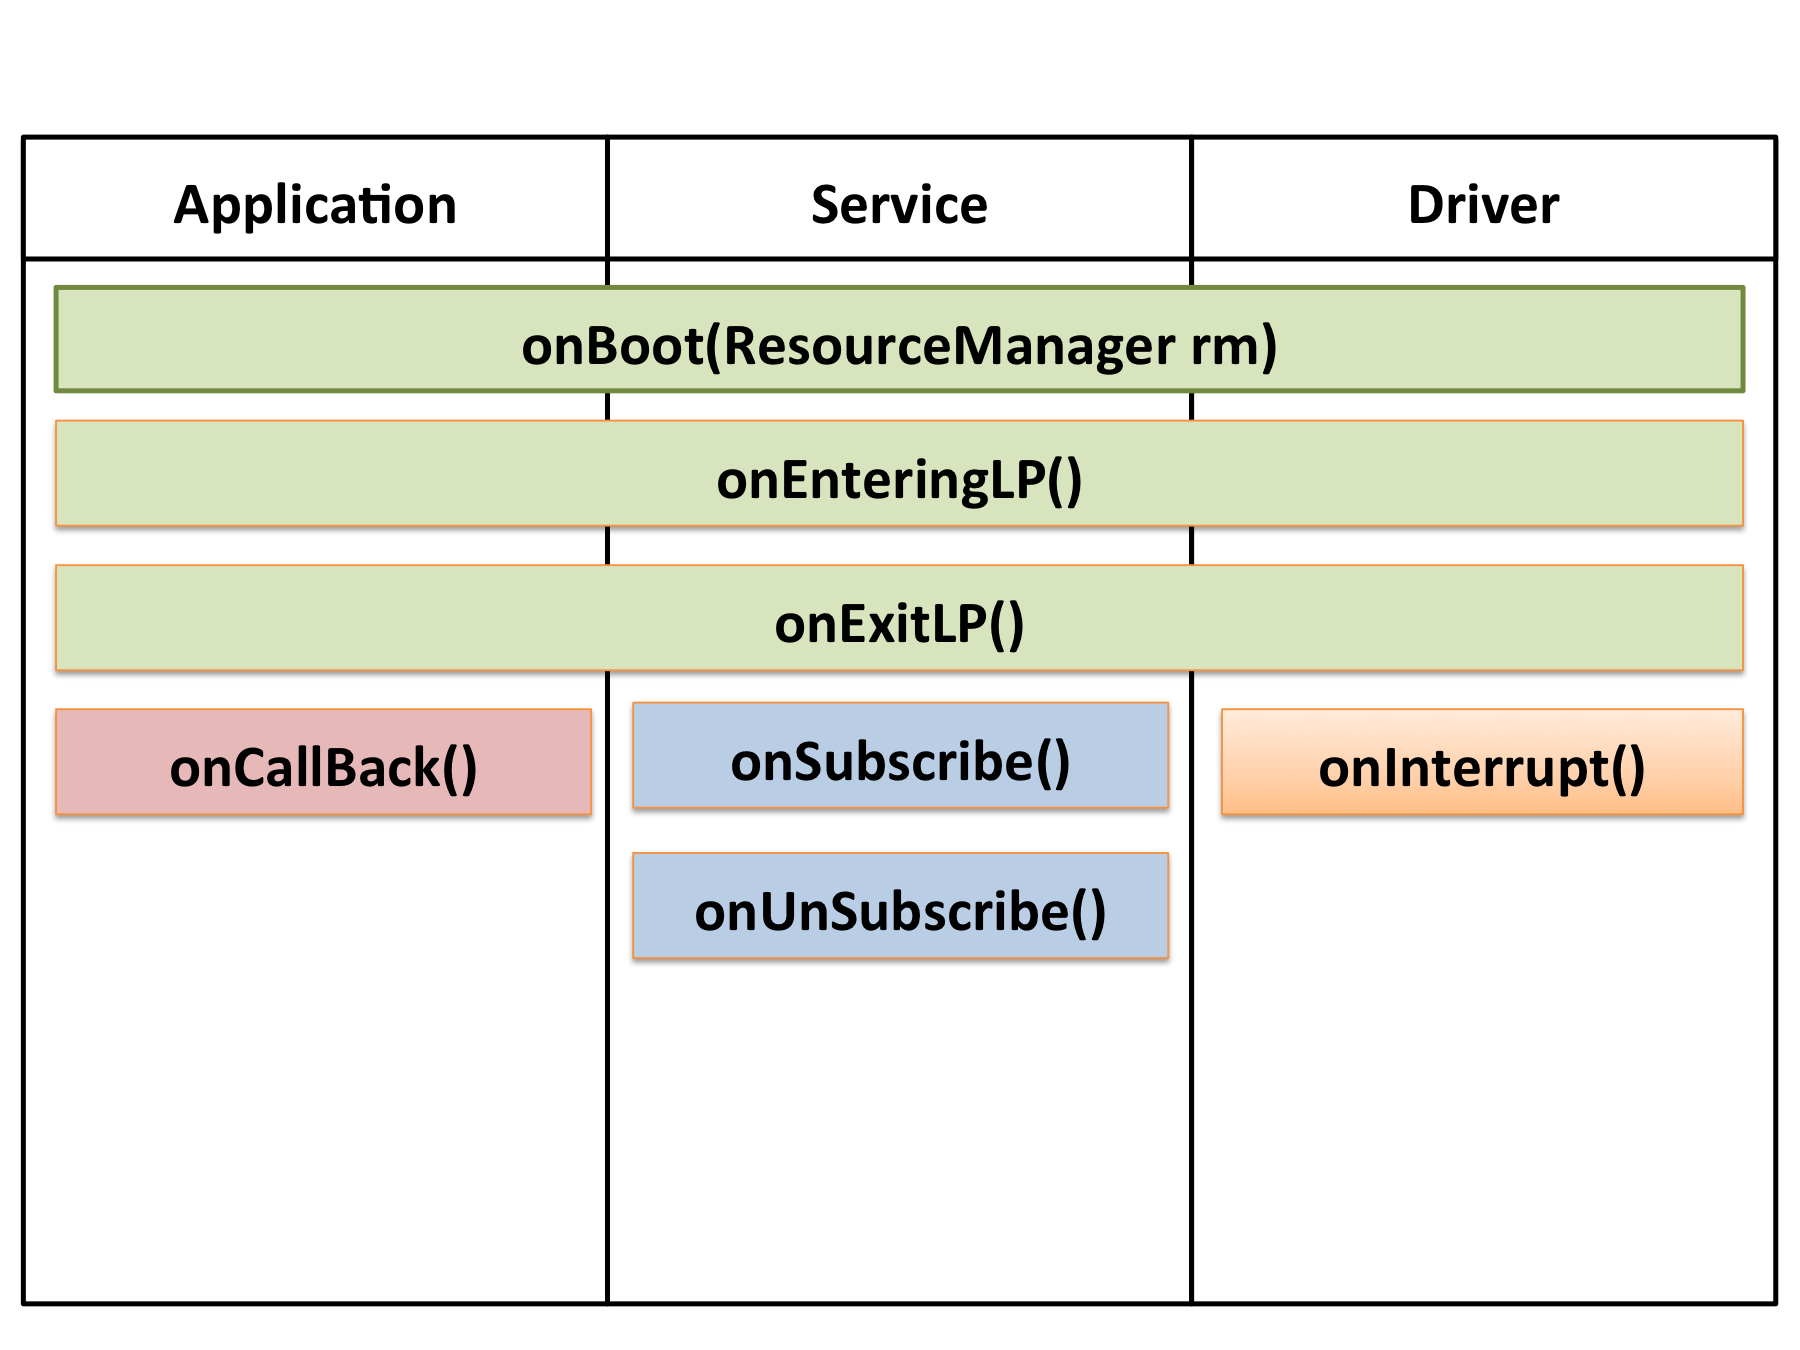
\includegraphics[width=1\columnwidth]{img/appcycle.png}
% % \caption{Runnable life cycle.}
% %  \label{fig:appcycle}
% % \end{figure}
% It's is not sufficient for a modern operating system allowing multiple
% simultaneous applications only have an event driven or preemptive
% multi-threading. In traditional OS the applications are not interrupted for
% longer period of times and in most of the cases there is no competition for
% resources. Resources need to be fairly distributed and applications, services or
% drivers notified upon event that effects program flow. Critical events are
% initialization of the application, the device is going to or waking up from low
% power mode as well secondary event like interrupts, timer, radio etc.
% % left here for event-driven e.g. Sergio add



\subsection{Loadable Applications and Drivers}
% should we talk about what tock does or jsut focut on the new generations of os
% instead? I prefere the considerations so there is no overlapp and
% inconsistencies in text

A modern operating system for embedded devices must support dynamically
loading new applications, the services they require, and drivers when new
peripherals are attached.
In embedded designs, new peripherals that require new custom drivers are
frequently added by neither core operating system developers nor peripheral
manufacturers. It is critical, then, that an operating system provide an
simple and safe means to add new drivers.

% to allow attache new
% peripherals and load they drivers, start new services, and load/unload
% applications. The OS is expected to be a full scale modern OS except it has to
% handle all of the constrain of OS for embedded devices. Unlike most desktop and
% server applications, embedded applications must continue to run without end-user
% intervention. There is no console to indicate to the user that an application
% has crashed. Even if a crash could be communicated to the user, there is little
% action they could take. While a Blue-Screen-Of-Death is annoying on a desktop or
% server, it is unacceptable in embedded systems. Moreover, given the variety of
% devices, the OS should allow developer to use any language supporting
% Application Binary Interface, ABI.



\subsection{Robust, Reliable, Safe and Efficient}

With resource sharing between applications and the end of exclusively trusted
software on embedded devices comes the need for better protection guarantees
from the operating system. The operating system must arbitrate and moderate
access to hardware resources and protect kernel memory from misbehaving
applications.  Further, embedded applications must continue to run without
end-user intervention as there is often little recourse for users to detect
and correct system error.


% % isolation incoming somewere here
% Besides separating drivers for core peripherals (SPI, USART, GPIO, etc) and
% device drivers (radio, flash, etc) into separate layers. Modern OS has to
% enforce safety policies not only on applications but also on device drivers. The
% OS has to ensure that at most one driver has access to a specific hardware
%  resource---multiplexing must be done explicitly in the core peripheral driver
%  or through an intermediate interface. Finally, the OS need to ensure that
%  device drivers cannot corrupt kernel memory or perform denial of service
%  attacks by drivers. Multiple application on the embedded device also requires
%  of to protect the kernel and other applications from malicious actions.

% While requirements have resemblance to those of a traditional OS, modern
% embedded OS has to fulfill them with the computational and energy constrains.

% energy efficency

% \name prevents drivers from subverting Rust's memory safety by restricting
% device drivers to a safe subset of the Rust language.~\endnote{Rust allows code
% to circumvent the type system using the \tt{unsafe} keyword. \name uses a
% compiler flag that disallows this keyword when compiling device drivers.} \name
% also ensures, at compile time, that at most one driver has access to a specific
% hardware resource---multiplexing must be done explicitly in the core peripheral
% driver or through an intermediate interface. Finally, \name ensures device
% drivers cannot corrupt kernel memory through careful choice of interfaces. \name
% ensures that \name does not protect the kernel from denial of service attacks by
% drivers. %wait what does this last sentence mean?




